%  LaTeX support: latex@mdpi.com 
%  For support, please attach all files needed for compiling as well as the log file, and specify your operating system, LaTeX version, and LaTeX editor.

%=================================================================
\documentclass[ijms,article,submit,moreauthors,pdftex]{Definitions/mdpi}
%\usepackage[table,xcdraw]{xcolor}

% For posting an early version of this manuscript as a preprint, you may use "preprints" as the journal and change "submit" to "accept". The document class line would be, e.g., \documentclass[preprints,article,accept,moreauthors,pdftex]{mdpi}. This is especially recommended for submission to arXiv, where line numbers should be removed before posting. For preprints.org, the editorial staff will make this change immediately prior to posting.

%--------------------
% Class Options:
%--------------------
%----------
% journal
%----------
% Choose between the following MDPI journals:
% ijms

%---------
% article
%---------
% The default type of manuscript is "article", but can be replaced by: 
% abstract, addendum, article, book, bookreview, briefreport, casereport, comment, commentary, communication, conferenceproceedings, correction, conferencereport, entry, expressionofconcern, extendedabstract, datadescriptor, editorial, essay, erratum, hypothesis, interestingimage, obituary, opinion, projectreport, reply, retraction, review, perspective, protocol, shortnote, studyprotocol, systematicreview, supfile, technicalnote, viewpoint, guidelines, registeredreport, tutorial
% supfile = supplementary materials

%----------
% submit
%----------
% The class option "submit" will be changed to "accept" by the Editorial Office when the paper is accepted. This will only make changes to the frontpage (e.g., the logo of the journal will get visible), the headings, and the copyright information. Also, line numbering will be removed. Journal info and pagination for accepted papers will also be assigned by the Editorial Office.

%------------------
% moreauthors
%------------------
% If there is only one author the class option oneauthor should be used. Otherwise use the class option moreauthors.

%---------
% pdftex
%---------
% The option pdftex is for use with pdfLaTeX. If eps figures are used, remove the option pdftex and use LaTeX and dvi2pdf.

%=================================================================
% MDPI internal commands
\firstpage{1} 
\makeatletter 
\setcounter{page}{\@firstpage} 
\makeatother
\pubvolume{1}
\issuenum{1}
\articlenumber{0}
\pubyear{2021}
\copyrightyear{2020}
%\externaleditor{Academic Editor: Firstname Lastname} % For journal Automation, please change Academic Editor to "Communicated by"
\datereceived{} 
\dateaccepted{} 
\datepublished{} 
\hreflink{https://doi.org/} % If needed use \linebreak
%------------------------------------------------------------------
% The following line should be uncommented if the LaTeX file is uploaded to arXiv.org
%\pdfoutput=1

%=================================================================
% Add packages and commands here. The following packages are loaded in our class file: fontenc, inputenc, calc, indentfirst, fancyhdr, graphicx, epstopdf, lastpage, ifthen, lineno, float, amsmath, setspace, enumitem, mathpazo, booktabs, titlesec, etoolbox, tabto, xcolor, soul, multirow, microtype, tikz, totcount, changepage, paracol, attrib, upgreek, cleveref, amsthm, hyphenat, natbib, hyperref, footmisc, url, geometry, newfloat, caption

%=================================================================
%% Please use the following mathematics environments: Theorem, Lemma, Corollary, Proposition, Characterization, Property, Problem, Example, ExamplesandDefinitions, Hypothesis, Remark, Definition, Notation, Assumption
%% For proofs, please use the proof environment (the amsthm package is loaded by the MDPI class).

%=================================================================
% Full title of the paper (Capitalized)
\Title{Investigating the molecular processes behind the cell-specific toxicity response to titanium dioxide nanobelts}

% MDPI internal command: Title for citation in the left column
\TitleCitation{Investigating the molecular processes behind the cell-specific toxicity response to titanium dioxide nanobelts}

% Author Orchid ID: enter ID or remove command
\newcommand{\orcidauthorA}{0000-0002-9454-4783} % Add \orcidA{} behind the author's name
\newcommand{\orcidauthorB}{0000-0002-5301-3142} % Add \orcidB{} behind the author's name
\newcommand{\orcidauthorC}{0000-0001-7542-0286} % Add \orcidC{} behind the author's name
\newcommand{\orcidauthorD}{0000-0002-7699-8191} % Add \orcidD{} behind the author's name

% Authors, for the paper (add full first names)
\Author{Laurent A Winckers $^{1}$\orcidA{}, Chris T Evelo $^{1,2}$\orcidB{}, Egon L Willighagen$^{1}$\orcidC{} and Martina Kutmon $^{1,2}$*\orcidD{}}

% MDPI internal command: Authors, for metadata in PDF
\AuthorNames{Laurent A Winckers, Chris T Evelo, Egon L Willighagen and Martina Kutmon}

% MDPI internal command: Authors, for citation in the left column
\AuthorCitation{Winckers, L.A,; Evelo, C.T; Willighagen, E.L.; Kutmon, M.}
% If this is a Chicago style journal: Lastname, Firstname, Firstname Lastname, and Firstname Lastname.

% Affiliations / Addresses (Add [1] after \address if there is only one affiliation.)
\address{%
$^{1}$ \quad Department of Bioinformatics - BiGCaT, NUTRIM School of Nutrition and Translational Research in Metabolism, Maastricht University\\
$^{2}$ \quad Maastricht Centre for Systems Biology (MaCSBio), Maastricht University}

% Contact information of the corresponding author
\corres{Correspondence: martina.kutmon@maastrichtuniversity.nl}

% Current address and/or shared authorship
%\firstnote{Current address: Affiliation 3} 
%\secondnote{These authors contributed equally to this work.}
% The commands \thirdnote{} till \eighthnote{} are available for further notes

%\simplesumm{} % Simple summary

%\conference{} % An extended version of a conference paper

% Abstract (Do not insert blank lines, i.e. \\) 
\abstract{Some engineered nanomaterials incite toxicological effects, but the underlying molecular processes are understudied. The varied physicochemical properties cause different initial molecular interactions, complicating toxicological predictions. Gene expression data allows us to study the responses of genes and biological processes. Overrepresentation analysis identifies enriched biological processes using the experimental data but prompts broad results instead of detailed toxicological processes. We demonstrate a targeted filtering approach to compare public gene expression data for low and high exposure on three cell lines to titanium dioxide nanobelts. Our workflow finds cell and concentration-specific changes in affected pathways linked to four Gene Ontology terms (apoptosis, inflammation, DNA damage and oxidative stress) to select pathways with a clear toxicity focus. 
We saw more differentially expressed genes at higher exposure, but our analysis identifies clear differences between the cell lines in affected processes. Colorectal adenocarcinoma cells showed resilience to both concentrations. Small airway epithelial cells displayed a cytotoxic response to the high concentration, but not as strongly as monocytic like cells. The pathway-gene networks highlighted the gene overlap between altered toxicity-related pathways. The automated workflow is flexible and can focus on other biological processes by selecting other GO terms.}

% Keywords
\keyword{nanomaterials; titanium dioxide; nanobelts; overrepresentation analysis; gene ontology; THP1; SAE; Caco2}

% The fields PACS, MSC, and JEL may be left empty or commented out if not applicable
%\PACS{J0101}
%\MSC{}
%\JEL{}

%%%%%%%%%%%%%%%%%%%%%%%%%%%%%%%%%%%%%%%%%%
% Only for the journal Diversity
%\LSID{\url{http://}}

%%%%%%%%%%%%%%%%%%%%%%%%%%%%%%%%%%%%%%%%%%
% Only for the journal Applied Sciences:
%\featuredapplication{Authors are encouraged to provide a concise description of the specific application or a potential application of the work. This section is not mandatory.}
%%%%%%%%%%%%%%%%%%%%%%%%%%%%%%%%%%%%%%%%%%

%%%%%%%%%%%%%%%%%%%%%%%%%%%%%%%%%%%%%%%%%%
% Only for the journal Data:
%\dataset{DOI number or link to the deposited data set in cases where the data set is published or set to be published separately. If the data set is submitted and will be published as a supplement to this paper in the journal Data, this field will be filled by the editors of the journal. In this case, please make sure to submit the data set as a supplement when entering your manuscript into our manuscript editorial system.}

%\datasetlicense{license under which the data set is made available (CC0, CC-BY, CC-BY-SA, CC-BY-NC, etc.)}

%%%%%%%%%%%%%%%%%%%%%%%%%%%%%%%%%%%%%%%%%%
% Only for the journal Toxins
%\keycontribution{The breakthroughs or highlights of the manuscript. Authors can write one or two sentences to describe the most important part of the paper.}

%%%%%%%%%%%%%%%%%%%%%%%%%%%%%%%%%%%%%%%%%%
% Only for the journal Encyclopedia
%\encyclopediadef{Instead of the abstract}
%\entrylink{The Link to this entry published on the encyclopedia platform.}
%%%%%%%%%%%%%%%%%%%%%%%%%%%%%%%%%%%%%%%%%%
\begin{document}
%%%%%%%%%%%%%%%%%%%%%%%%%%%%%%%%%%%%%%%%%%
%\setcounter{section}{-1} %% Remove this when starting to work on the template.
\section{Introduction}

Engineered nanomaterials have become important in our daily life as they are utilized in the fields of food, packaging, cosmetics, drug and vaccine delivery, and many others~\cite{Ray2009}. For example, silver and carbon nanotubes are used in a variety of cleansers because of their antimicrobial properties, and silicon dioxide is used as a food additive as it decreases viscosity and regulates acidity~\cite{Shin2015}. Nevertheless, some nanomaterials, such as asbestos fibres and silica dust, show how small particles can cause adverse outcomes to those exposed to them~\cite{Visona2018,Markowitz2015,Chen2012,Arnoldussen2019}.

The detailed biological processes related to the toxicity of many engineered nanomaterials are not all yet fully understood~\cite{Podila2012,Bahadar2016}. Due to the varied physicochemical properties of nanomaterials and often even of the particles within the nanomaterial itself, it is difficult to predict the biological effects leading to toxicity. Biological response and toxicity depend on the size of the nanoparticle itself, size of the agglomerate, surface impurities, and degradability~\cite{DeStefano2012}. Furthermore, other things that have an effect on the biological response and toxicity include the way of exposure, the entry route into the human body, and the distribution in the body have an effect on the biological response and toxicity~\cite{Shin2015}. The shape of a nanoparticle also has an influence on the nanoparticle’s effects, where for example nanobelts, a nanostructure in the form of a belt, shown to be more pro-inflammatory compared to spheres~\cite{Silva2013}. Studies have found that there are various biological effects and toxicity of engineered nanomaterials under different circumstances and with varying engineered nanomaterials~\cite{Ray2009,Atha2017,Donaldson2003,Sung2008,EbabeElle2013}. These changes in biological effects are ascribed to the differences in chemical and physical properties of nanomaterials. However, studying the property – biological effect relation is complicated because of the difficulty to create identical nanomaterials from different batches and/or sources due to the varying physicochemical properties of nanomaterials~\cite{Mulhopt2018}.Nevertheless, manually curation of transcriptomics datasets regarding nanomaterials are done to enhance their degree of FAIRness to aid nanomaterial safety assessment~\cite{AliisaSaarimaki}.  

Furthermore, a relatively well-studied and widely used nanomaterial is titanium dioxide (TiO\textsubscript{2}). Due to its general properties, such as the photocatalytic activity and white color, it is used in various applications such as (photo)catalysis, antibacterial agents, and consumer products. Whereas TiO\textsubscript{2} particles are shown not to be able to penetrate through the skin, entry into the body can happen via inhalation or ingestion where it then has to pass the gastrointestinal tract~\cite{Shakeel2015,Gupta2018}. 

Regarding the adverse outcomes, the toxic effects of TiO\textsubscript{2} are known to happen in order, like most toxicity related biological processes. TiO\textsubscript{2} is known to induce reactive oxygen species production which involves lipid peroxidation and eventually will lead to cell damage and DNA damage~\cite{Hou2019,LAzou2008}. Furthermore, The increase in oxidative stress can contribute to the promotion of apoptosis of the affected cells~\cite{Circu2010,Redza-Dutordoir2016}. Consequently, TiO\textsubscript{2} nanoparticles have been shown to induce inflammation~\cite{Yan2020,Baisch2014} among other things via the aforementioned oxidative stress in mammalian cells~\cite{Hou2019,Meena2015}. It has been shown that TiO\textsubscript{2} nanoparticle exposure can lead to impaired immune homeostasis including increases in TNF-$\alpha$, IFN-$\gamma$, IL-2, IL-4, IL-6, IL-8, and IL-10 secretion~\cite{RothenRutishauser2007,Bettini2017,MedinaReyes2015}. 

To study the detailed mechanisms of the cellular response, bioinformatics and systems biology approaches, including pathway and network analysis, were used to assess the effects on toxicity-related processes upon exposure to TiO\textsubscript{2}-nanobelts, \textit{i.e.} reactive oxygen species formation and oxidative stress, apoptotic cell death, inflammation, and DNA damage~\cite{Zhang2018,Liu2019}. Pathway enrichment analysis helps to put high-throughput omics data such as transcriptomics into a biological context~\cite{Khatri2012} and the visual diagrams from pathway databases such as WikiPathways~\cite{Martens2020} and Reactome~\cite{Fabregat2017} provide a way to visualize the effects on cellular processes. However, navigating all the affected pathways and the roles of the genes in these pathways can be nontrivial: genes can participate in multiple pathways, and pathways tend to overlap with each other. Moreover, we want to be able to focus on detailed, molecular pathways related to a specific biological process, such as apoptosis, inflammation, DNA damage, and oxidative stress. Overrepresentation, with respect to these processes alone, makes it possible to focus on a subset of genes, but it does not have the link to the pathways. Instead, we selected pathways based on their gene overlap with specific GO-terms covering toxicity-related biological processes and subsequently used the overrepresentation of differentially expressed genes to select relevant pathways out of this subset. We further studied these results in detail using network analysis approaches to investigate pathway overlap and crosstalk.

In this study we re-examined a publicly available dataset generated by Tilton~\textit{et al.}~\cite{Tilton2013} (accession number: GSE42069)~\cite{Edgar2002} to study the detailed molecular mechanisms of TiO\textsubscript{2}-nanobelts toxicity. We analyzed gene expression data from three different cell lines exposed to either one of two concentrations of TiO\textsubscript{2}-nanobelts for 24 hours. The cell lines used were human primary small airway epithelial cells (SAE), human monocytic cells (THP1), and human epithelial colorectal adenocarcinoma cells (Caco2). These cell lines represent three common areas of exposure in the human body \textit{i.e.} skin epithelium, colon epithelium, and the innate immune system that typically will respond to particles that entered the body. We aim to provide an overview of the dose-dependent and cell type-specific response by focusing on toxicity-related processes. Apart from a significant increase in the activity of toxicity-related processes after exposure with a higher dosage, differences in intensity, and affected processes might occur between the cell lines. Using this work as an example, we will discuss the toxicological effects of TiO\textsubscript{2} nanobelts on the three cell lines and the importance and benefits of analysis workflows in the nanomaterial research field.
 
%%%%%%%%%%%%%%%%%%%%%%%%%%%%%%%%%%%%%%%%%%
\section{Results and Discussion}

\subsection*{Differential gene expression}
The differential gene expression analysis for the three cell lines after exposure to two different TiO\textsubscript{2}-nanobelt concentrations show that a high concentration of TiO\textsubscript{2}-nanobelts (Figure~\ref{fig:fig1}, right column) causes stronger gene expression changes in all three cell lines than at a low concentration (Figure~\ref{fig:fig1}, left column). While the Caco2 and SAE cells also show an increased response to the high TiO\textsubscript{2}-nanobelts concentration, the THP1 cells respond much stronger to the high concentration in terms of differentially expressed genes passing our criteria. Dose-dependent increases in response have been shown for many nanomaterials~\cite{Iavicoli2018,Ding2005}.

\begin{figure}[ht!]
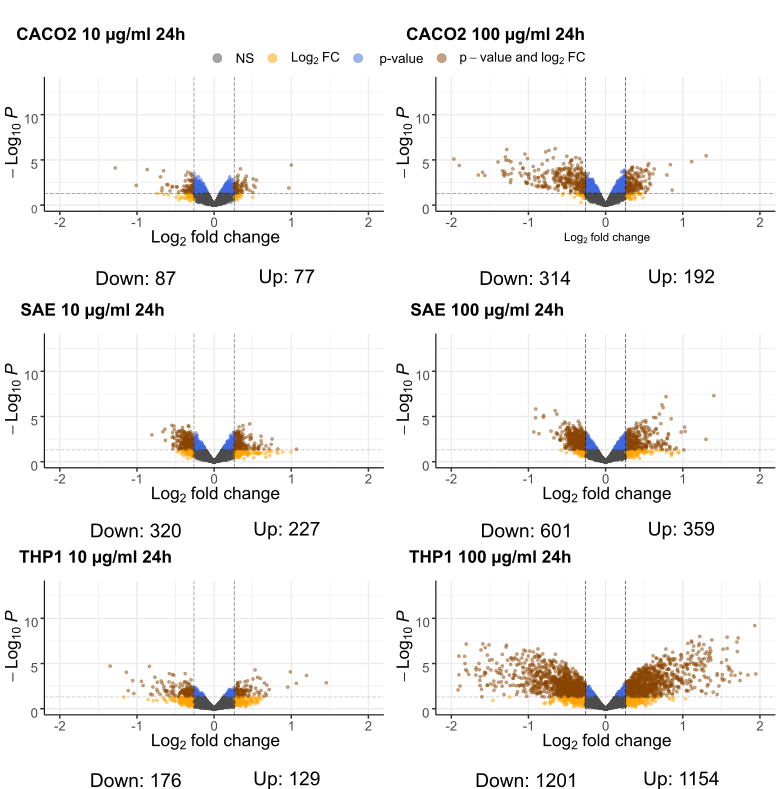
\includegraphics[width=0.9\linewidth]{fig1.png}
  \caption{Gene expression volcano plots for different cell lines and TiO\textsubscript{2}-nanobelts concentrations.
   On the x-axis log\textsubscript{2}(fold change) is depicted whereas on the y-axis the -log\textsubscript{10}(p-value) is depicted. The dotted lines represent cut-off values for significantly changed genes (log\textsubscript{2} fold change $>$ 0.26 or $<$ -0.26, p-value $<$ 0.05). Brown color depicts that a gene meets both cut-off criteria, a blue color relates to meeting only the p-value cut-off, an orange color relates to meeting only the log2 fold change cut-off and grey color indicates that a gene does not meet any of the criteria.}
\label{fig:fig1}
\end{figure}

\subsection*{Pathway analysis}
Using the differentially expressed genes from the different cell lines, overrepresentation analysis was performed to identify altered pathways after TiO\textsubscript{2}-nanobelt exposure. The number of significantly overrepresented pathways (p-value $<$ 0.05) are shown in Table 1 in the column “Significant”. Concordant to the increase in differentially expressed genes matching our criteria shown in Figure 1, the number of resulting pathways increases with a surge in the concentration of TiO\textsubscript{2}-nanobelts. However, there was a smaller increase in differentially expressed genes, we found a similar increase in resulting pathways for the SAE cell line. While there was also an increase in the number of genes found for the Caco2 cell lines it did not directly translate to an increase in overrepresented pathways. Although over-representation analysis provides a great overview of all processes that are affected, it takes time to go manually over the many overrepresented pathways. Therefore, an automated method to select desired pathways, \textit{i.e.} toxicity-related pathways, gives a new approach to interpret the data. 

\subsection*{Toxicity-related pathways}
To gain more insight into the toxicity-related processes, the overrepresented pathways were further categorized into pathways related to apoptotic process, inflammatory response, DNA damage response, and/or oxidative stress. Often this kind of clustering of the pathways is done manually. However, we implemented a gene-based approach. First, gene sets of four Gene~Ontology~(GO) terms were obtained, \textit{i.e.} “apoptotic process”~(GO:0006915, 1269 genes), “inflammatory response”~(GO:0006954, 569 genes),  “cellular response to DNA damage stimulus”~(GO:0006974, 762 genes), and “response to oxidative stress”~(GO:0006979, 243 genes). Evidently, these processes are tightly connected. Whereas some can be causative for others, they are expected to overlap.  Additional file A1 shows the gene overlap between the four GO gene sets in a Venn-diagram (see Additional file A1). Next, we calculated the gene overlap between the pathways from the WikiPathways pathway collection with the annotated genes of the four GO-terms. The overlap was calculated by dividing the number of toxicity-related genes present in the pathway by total number of genes present in the pathway. As a cut-off we used 50$\%$ indicating that at least half of the pathway is directly linked to GO-term of interest via their gene overlap.

To select the desired gene overlap cut-off, we compared four cut-offs with each other and an overrepresentation analysis approach to see how many pathways these would give. The cut-offs we used were 50\%, 60\%, 70\% and 80\%. For the overrepresentation analysis we looked for overrepresentation of the pathway genes in the gene lists of the GO-terms. The results are shown in Table~A2 (see Additional file A2). The overrepresentation analysis (p-value < $<$ 0.05) showed the most pathways to be linked to the four GO-terms, in this case it showed 401, 250, 203 and 205 pathways overrepresented for the apoptotic process, inflammatory response, DNA damage and oxidative stress GO-terms respectively. The 80\% and 70\% gene overlap resulted in almost similar amounts of pathways compared to each other. They even resulted in 0 pathways for the inflammatory response GO-term. Moreover, it stands out that for the gene overlap approach only one pathway meets at least 50\% or higher gene overlap with the oxidative stress GO-term. Additionally, it is interesting to see that an overrepresentation analysis prompts hundreds of pathways compared to just dozens when looking at gene overlap. Comparing the results of the overrepresentation analysis and various cut-offs the at least 50\% gene overlap cut-off was deemed best for our approach. 

After this filtering step we found, out of the 1,076 pathways in the human pathway collection, 66 pathways are related to the apoptotic process, 15 are linked to inflammatory response, and 28 are linked to DNA damage and 2 are linked to oxidative stress.
It is noticeable that there are only two oxidative stress pathways, \textit{i.e.} Detoxification of Reactive Oxygen Species~(wikipathways:WP2824~\cite{WP2824}) and Oxidative Stress~(wikipathways:WP408~\cite{WP408}), that have at least 50$\%$ of their genes overlapping with the genes annotated to the GO-term "response to oxidative stress". Based on this finding we can argue that most pathways in the pathway database we have used describe different processes which result in oxidative stress or where oxidative stress is part of/has an influence on the process itself. Whereas these do not describe oxidative stress as a process.  Nevertheless, these pathways are of interest for our analysis. 

\subsection*{Study effect on toxicity-related pathways}
The number of altered toxicity-related pathways is shown in Table 1. The overrepresentation analysis was performed using the differentially expressed genes (log2 fold change lower than -0.26 or greater than 0.26 and p-value lower than 0.05). 

The Caco2 cell line shows for both concentration 10 overrepresented pathways. While the SAE cell line shows 3 for the low concentration, which could be an indication of a very little toxic response to the TiO\textsubscript{2}-nanobelts exposure, and 15 for the high concentration. The THP1 cell line shows a clear toxic response activation for the high concentration with 39 overrepresented pathways, and 10 for the low concentration.


\begin{table}[]
\caption{Table depicting the number of significantly overrepresented pathways, altered toxicity pathways and the number of altered toxicity pathways for each GO-term.}
\resizebox{\columnwidth}{!}{%
\begin{tabular}{lcc|cccc}
 & \textbf{Significant} & \textbf{Toxicity} & \textbf{Apoptosis} & \textbf{Inflammation} & \textbf{\begin{tabular}[c]{@{}c@{}}DNA \\ damage\end{tabular}} & \textbf{\begin{tabular}[c]{@{}c@{}}Oxidative \\ stress\end{tabular}} \\ \hline
\textbf{Pathways} & 1076 & 101 & 66 & 15 & 28 & 2 \\ \hline
Caco2 low & 56 & 10 & 5 & 0 & 5 & 0 \\
Caco2 high & 58 & 10 & 10 & 1 & 0 & 0 \\ \hline
SAE low & 28 & 3 & 1 & 0 & 2 & 0 \\
SAE high & 50 & 15 & 6 & 1 & 8 & 0 \\ \hline
THP1 low & 38 & 10 & 9 & 4 & 0 & 0 \\
THP1 high & 201 & 39 & 31 & 9 & 3 & 1 
\end{tabular}%
}
\end{table}


Importantly, while molecular pathways describe a process on a detailed level, their boundaries are often not clearly defined. Pathways are not independent, and they interact with each other through shared genes or sub-pathways. Figure~\ref{fig:fig2} shows the gene overlap between the altered toxicity-related pathways in pathway-gene networks and highlights the differences in response between the cell lines. Pathways that cluster together indicate that these pathways depict similar biological processes with a high gene overlap. In the following sections, the biological pathways affected in the different cell lines will be discussed in detail.


\begin{figure}[ht!]
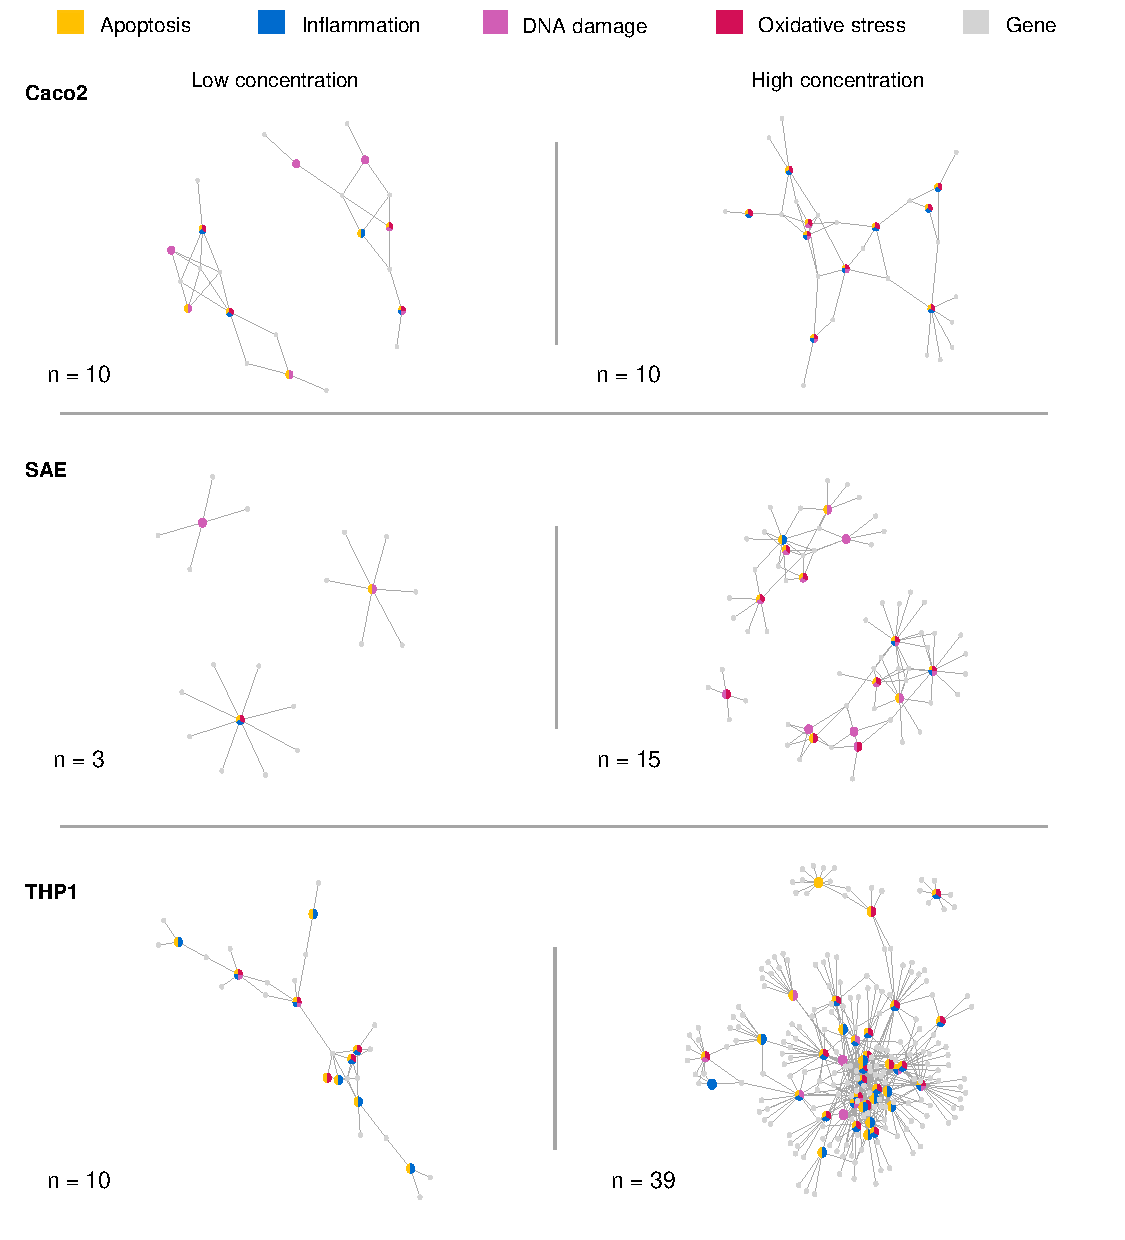
\includegraphics[width=0.9\linewidth]{fig2.pdf}
  \caption{Pathway-gene networks of altered toxicity-related pathways.
   Color of the nodes depict to which GO-term the pathway is affiliated. Orange depicts apoptosis, blue depicts inflammation, pink depicts DNA damage and bordeaux depicts oxidative stress. Gray nodes represent genes. Number (n) represents the number of significantly overrepresented pathways that are depicted in the networks.}
\label{fig:fig2}
\end{figure}


\subsection*{Caco2 cells}
While for both concentrations the Caco2 cell line shows the same number of overrepresented pathways, the pathways compared between the low- and high concentration are not all the same. Of the ten pathways, three are found for both concentration, namely IL-5 Signaling Pathway (wikipathways:WP127,~\cite{WP127}), IL-2 Signaling Pathway (wikipathways:WP49,~\cite{WP49}) and Endometrial cancer (wikipathways:WP4155,~\cite{WP4155}). Interestingly to see is that for the low concentration pathways related to DNA-damage and repair show up in the results. For example, HDR through Homologous Recombination (HRR) or Single Strand Annealing (SSA) (wikipathways:WP3567,~\cite{WP3567}), Nonhomologous End-Joining (NHEJ) (wikipathways:WP3550,~\cite{WP3550}) and DNA Double Strand Break Response (wikipathways:WP3543,~\cite{WP3543}) are amongst these pathways. While for the high concentration it is interesting to see that the Apoptosis pathway (wikipathways:WP254,~\cite{WP254}) shows up. Which could be an indication of Caco2 cells possibly undergoing apoptotic processes upon exposure to TiO\textsubscript{2}-nanobelts. However, These results indicate that the studied processes in Caco2 cell lines are not extensively affected by the administration of TiO\textsubscript{2}-nanobelts, for either the low or the high concentration. This finding supports the conclusion based on the cell viability assay results in the original study which showed that there was no significant decrease in cell viability for the Caco2 cell line for both concentrations of TiO\textsubscript{2}-nanobelts~\cite{Tilton2013}. 

\subsection*{SAE cells}
For the SAE cell line, the low concentration only prompted three overrepresented pathways compared to 15 for the high concentration. Noticeable as well, only one of those three pathways was found to be overrepresented for the high concentration as well, namely HDR through Homologous Recombination (HRR) or Single Strand Annealing (SSA) (wikipathways:WP3567,~\cite{WP3567}). This increase in pathways with a significantly increased overrepresentation of affected genes is an indication that upon exposure to the high concentration of TiO\textsubscript{2}-nanobelts more biological processes related to toxicity are affected compared to the low concentration. 

Next, for the SAE cell line exposed with the low concentration, we found three overrepresented pathways. As for the high concentration we found 15 overrepresented pathways. This increase in pathways with a significantly increased overrepresentation of affected genes is an indication that more biological processes related to toxicity are affected compared to the low concentration upon exposure to the high concentration of TiO\textsubscript{2}-nanobelts . For the low concentration the pathways HDR through Homologous Recombination (HRR) or Single Strand Annealing (SSA) (wikipathways:WP3567,~\cite{WP3567}), IL-6 signaling pathway (wikipathways:WP364,~\cite{WP364}) and Regulation of TP53 Activity through Phosphorylation (wikipathways:WP3838,~\cite{WP3838}) are overrepresented. The first pathway describes a process of DNA double strand break repair, where the second pathway is described the signaling of the cytokine IL-6 and the last pathway described the regulation op TP53. Except for the first pathway, which is also found in the result for the high concentration, the overrepresented pathways describe more general regulatory pathways rather than detailed process describing pathways. However, for the high concentration we see multiple pathways related to DNA damage, such as the aforementioned HDR through Homologous Recombination (HRR) or Single Strand Annealing (SSA) (wikipathways:WP3567,~\cite{WP3567}), DNA IR-damage and cellular response via ATR (wikipathways:WP4016,~\cite{WP4016}), DNA IR-Double Strand Breaks (DSBs) and cellular response via ATM (wikipathways:WP3959,~\cite{WP3959}) and DNA Mismatch Repair (wikipathways:WP531,~\cite{WP531}) among others. Moreover, The results prompted apoptosis related pathways such as Apoptosis Modulation and Signaling (wikipathways:WP1772,~\cite{WP1772}) and Apoptosis Modulation by HSP70 (wikipathways:WP384,~\cite{WP384}). This is also an indication that the high concentration induced more distinct biological processes related to toxicity compared to the low concentration for the SAE cell line. 

\subsection*{THP1 cells}
For the THP1 cell line, there are only 10 significantly overrepresented pathways for the low concentration of TiO\textsubscript{2}-nanobelts. However, among these pathways, the pathways TNF signaling (wikipathways:WP3380,~\cite{WP3380}), Apoptosis (wikipathways:WP254,~\cite{WP254}), Apoptotic execution phase (wikipathways:WP1784,~\cite{WP1784}), TNF alpha Signaling Pathway (wikipathways:WP231,~\cite{WP231}) and TNF related weak inducer of apoptosis (TWEAK) Signaling Pathway (wikipathways:WP2036,~\cite{WP2036}) are present. This indicates that upon exposure to the low concentration of TiO\textsubscript{2}-nanobelts the THP1 cell line activates immune and inflammation-related processes. This result can be explained as a general cell activity response since THP1 is a macrophage-like cell line. However, it can also be explained due to the effect of TiO\textsubscript{2}-nanobelts on the THP1 cell line in this case. TiO\textsubscript{2}-nanobelts are likely to induce toxic processes, even at a low concentration, which results in an inflammatory response of the THP1 cells. Similar inflammatory responses, like activation of Nf-$\kappa$B and production of TNF-$\alpha$, were seen in these cells upon exposure to other nanoparticles such as ZnO NM-110, SiO\textsubscript{2} NM-200 and Ag NM-300~\cite{Brzicova2019}. 

Compared to the low concentration, the high concentration yields more pathways with significant overrepresentation \textit{i.e.} 39 versus 10. Except for the pathway Apoptotic execution phase (wikipathways:WP1784,~\cite{WP1784}) all other 9 pathways which showed up for the low concentration were found for the high concentration as well. In addition to these pathways, pathways such as Oxidative Stress (wikipathways:WP408,~\cite{WP408}), Nanoparticle triggered regulated necrosis (wikipathways:WP2513,~\cite{WP2513}) and Mismatch Repair (wikipathways:WP3381,~\cite{WP3381}) and more were among the significant pathways. These results indicate that the THP1 cell line upon exposure to the high concentration of TiO\textsubscript{2}-nanobelts results in toxicity-related processes such as inflammation, DNA damage, and oxidative stress. The higher number of pathways that show up in the result together with the biological processes they depict indicate that the high concentration induces greater effects than the low concentration. This was also seen in the original paper where the low concentration induced a significant decrease in cell viability, while the high concentration induced an even greater decrease~\cite{Tilton2013}. Furthermore, it has also been shown that nanoparticles can activate similar processes, such as inflammatory processes and DNA damage, as seen upon exposure to the high concentration~\cite{Brzicova2019,Huang2017}.

\subsection*{Comparison between cell lines}
The focused analysis of alterations in toxicity-related processes showed differences between the three cell lines and the concentrations studied. It has been reported before that the molecular response depends on the cell type and concentration~\cite{TadaOikawa2016}. 

Caco2 cells seem resilient to the exposure and show very little activation of toxicity-related processes. The passage of nanoparticles through the cellular barriers of Caco2 cells has been shown to be limited which could result in reduced uptake and therefore less toxic response~\cite{Ye2017}. Subsequently, this indicates a lower importance of gastro-intestinal uptake in general. On the other hand, TiO\textsubscript{2}-nanobelts caused the biggest toxicological response to THP1 cells,as they are more sensitive to exposure compared to epithelial cell lines RLE-6TN and BEAS-2B~\cite{Xia2013}. Moreover, it has been reported that this response is specific to the nanobelt form of TiO\textsubscript{2}~\cite{Xia2013}.

Interestingly, approximately 10\% of the pathways in WikiPathways and Reactome can be categorized as toxicity-related, in other words these pathways have a t least 50\% gene overlap with the GO-terms we selected. This highlights the fundamental cellular processes involved but could also indicate a bias in the pathway collections towards these well-studied processes. Nonetheless, these pathways are considered important pathways, hence they are studied well.  

To illustrate how the effects can be studied in more depth we visualized the log fold change of all six conditions on the Oxidative Stress pathway (wikipathways:WP408~\cite{WP408}), the Apoptosis pathway (wikipathways:WP254~\cite{WP254}) and the DNA Mismatch Repair pathway (wikipathways:WP531~\cite{WP531}). It shows that for most genes in these pathways gene expression data is present (see Additional file A3 and A4). 

While the Oxidative Stress pathway shown in Figure~\ref{fig:fig3}, only shows up to be significantly overrepresented for the THP1 cell line for the high concentration it is still an interesting pathway to dive deeper into. The NFKB1 gene, which encodes for the Nf$\kappa$B-p105 subunit, has the highest log fold change for the THP1 cell line, high concentration. Additionally, the THP1 cell line, low concentration shows a positive log fold change as well, whereas the SAE cell line shows negative log fold changes and the Caco2 cell line noticeably lower positive log fold changes for both concentrations. Furthermore, the SOD2 gene, which is involved in the conversion of superoxide and protects against oxidative stress, shows a similar pattern~\cite{Urso2003}. These genes indicate that the THP1 cell line responds to oxidative stress by increasing the expression of protective genes. 

\begin{figure}[ht!]
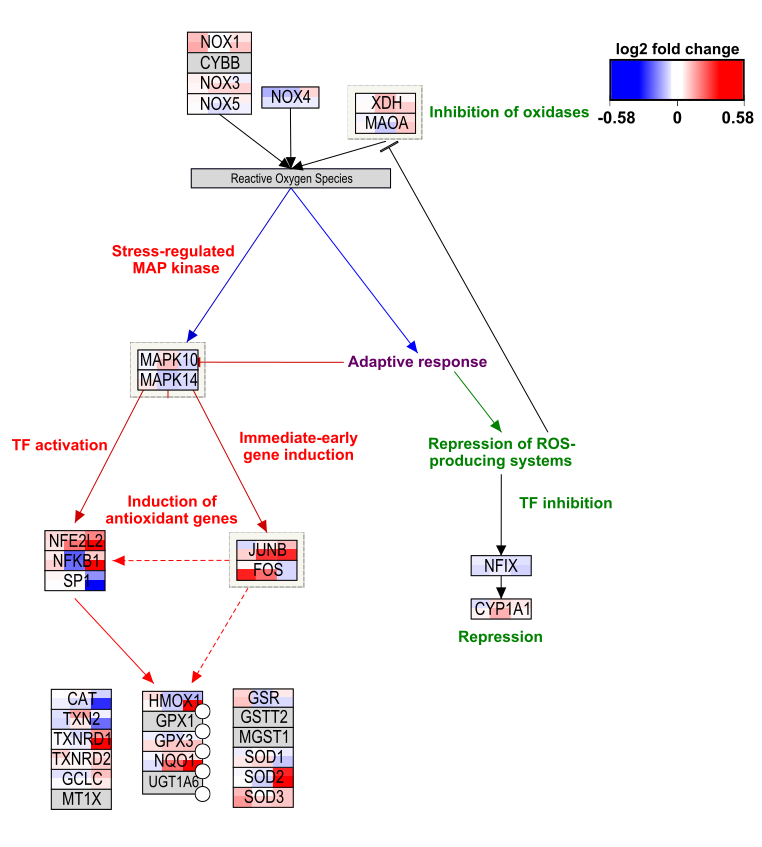
\includegraphics[height=12cm,keepaspectratio]{fig3.png}
  \caption{Visualization of log fold change on the Oxidative Stress pathway (wikipathways:WP408) for all six conditions.
   Cell lines are depicted from left to right as Caco2, SAE and THP1. The top row depicts the low concentration whereas the bottom row depicts the high concentration. Gradient goes from blue (log fold change $<$ -0.58) via white (log fold change = 0.0) to red (log fold change $>$ 0.58).
}
\label{fig:fig3}
\end{figure}

Moreover, the Apoptosis pathway shows positive log fold changes of the CASP2 and CASP7 genes, which are involved in apoptosis execution, for the SAE and THP1 cell lines for both concentrations whereas the Caco2 cell line shows no negative or positive log fold change~\cite{BouchierHayes2011,Lamkanfi2010}. Furthermore, the pathway shows positive log fold changes for the apoptosis promoting interferon regulatory factors such as IRF4 and IRF5~\cite{Stang2007,Fanzo2003,Hu2009}, which is a similar pattern as described for the CASP2 and CASP7 genes. This could be an indication that apoptosis is stimulated in these cell lines. However, the original study by Tilton \textit{et al.} does not show a significant decrease in cell viability. 
The DNA Mismatch Repair pathway shows a positive log fold change for the Caco2 THP1 cell lines for the LIG1 gene, which encodes for DNA ligase 1. This enzyme is involved in both DNA replication and in this context more importantly repair~\cite{Mota2019}. The aforementioned genes show positive log fold changes for the THP1 cell line throughout the pathway. The increase in expression of these genes could be an indication that DNA mismatch repair is activated due to exposure to TiO\textsubscript{2}-nanobelts.

\subsection*{The advantage of our approach}
Enrichment analysis for gene expression data is well-established and can be easily automated to increase reproducibility~\cite{Yu2012}. The interpretation of the long list of altered, often overlapping pathways is still a challenge. By providing an automated approach to filter the pathway enrichment result towards a specific biological focus, in this case toxicity, a more context-specific interpretation is facilitated. The generated pathway-gene networks showcase the connectedness of the processes and provide a more systemic view than looking at individual pathways. In addition, the approach yields a fast and easy method to select pathways of interest for more detailed scrutiny as we have shown. While interpretation and comparison between multiple datasets on a process level are still challenging, the automated analysis workflow used supports the exploration of the data~\cite{TiO2-scripts}.

%%%%%%%%%%%%%%%%%%%%%%%%%%%%%%%%%%%%%%%%%%
\section{Conclusions}

This study investigated the molecular response of three different cell lines to exposure to TiO\textsubscript{2}-nanobelts. Using our process-level analysis based on pathway analysis, pathway selection using gene sets, and network visualization, our findings support the results by S.C. Tilton \textit{et al.} showing that the three cell lines, Caco2, SAE, and THP1, show different toxicity-related responses to the exposure of TiO\textsubscript{2}-nanobelts from resilient Caco2 and SAE cells to strongly responding THP1 cells. The latter is not unexpected since the observed effects align with the biological function of these immune cells. Importantly, the approach allowed us to not just find changes in gene expression, but also responding molecular pathways via the pathway analysis and, additionally, allows us to filter the broad pathway enrichment results to a focused view on the cytotoxic processes affected. This allows us to visualize and explore the interactions between responding genes, based on underlying molecular processes. This versatile approach captured in the R-script can be easily adapted to isolate other processes by using other Gene Ontology terms diverting the focus to other biological processes of interest.

%%%%%%%%%%%%%%%%%%%%%%%%%%%%%%%%%%%%%%%%%%
\section{Materials and Methods}

\subsection*{Dataset}
In this study, a published and publicly available transcriptomics dataset generated by Tilton~\textit{et al.}~\cite{Tilton2013} was used. The dataset is available from the Gene Expression Omnibus (accession number: GSE42069)~\cite{Edgar2002}. Quality control, data pre-processing, and statistical analysis were performed using scripts from ArrayAnalysis.org~\cite{Eijssen2013}. 

The dataset consisted of 18 samples from three human-like cell lines, \textit{i.e.} Caco2, SAE, and THP1, which were exposed to either medium (control), 10~$\mu$g/ml or 100~$\mu$g/ml TiO\textsubscript{2}-nanobelts for 24 hours in triplicate. Culture conditions were kept as identical as possible between the three cell lines. Details can be found via the original publication by Tilton~\textit{et al.}~\cite{Tilton2013}.

Volcano plots depicting differential gene expression were made using EnhancedVolcano package (version 1.4.0) for R (version 3.6.1)~\cite{R2020,VolcanoPlot}. Genes were considered differentially expressed between treated and control when they had an absolute fold change greater than 1.2 (log2 fold change lower than -0.26 or higher than 0.26) and a p-value lower than 0.05. 

\subsection*{Pathway analysis}
Overrepresentation analysis was performed using the enricher function of the clusterProfiler package (version 3.14.3)~\cite{Yu2012} for R to identify the molecular changes on a pathway level. The human pathway collection containing 1076 pathways was obtained from WikiPathways (http://www.wikipathways.org, version 20201003,~\cite{Martens2020}). The Curated and Reactome collections from WikiPathways were included in the analysis. Enrichment analysis was performed differentially expressed genes using the fold change and p-value cutoff as described in the previous section. Additionally, default settings of the enricher function of the clusterProfiler package were used except p-value and q-value (false discovery rate) cutoff were set to 1 to include all results at this stage. This allows us to later select the desired results based on a p-value smaller than 0.05. Minimal gene set size was set to 10 and the maximum gene set size was set to 300.

\subsection*{Toxicity-related processes}
Within the two human pathway collections used, toxicity-related pathways were identified based on the gene overlap with the toxicity-related gene sets. The overlap was calculated by dividing the number of toxicity-related genes present in the pathway by total number of genes present in the pathway. The gene sets were retrieved from the Gene Ontology (GO, version: release 2020-06) for the following four toxicity-related GO-terms: “apoptotic process” (GO:0006915), “inflammatory response” (GO:0006954), “cellular response to DNA damage stimulus” (GO:0006974) and “response to oxidative stress” (GO:0006979)~\cite{Ashburner2000,Carbon2020}. Associated genes were retrieved using the biomaRt package in R (version 2.42.0, Ensembl Genes 100)~\cite{Durinck2005,Durinck2009}. Using the GO evidence codes, only genes with experimental evidence or manually curated annotations were included to ensure high confidence that the gene is involved in the specific process (IBA, IC, IDA, IEP, IGI, IMP, IPI, TAS, http://geneontology.org/docs/guide-go-evidence-codes/, see Additional file A5). Gene overlap between GO-terms was visualized using Venny version 2.1.0~\cite{Venny}. 

\subsection*{Network visualization}
Altered pathways in the enrichment analysis were filtered for toxicity-related pathways and then visualized as pathway-gene networks to portray the overlap and crosstalk between the pathways. To construct the networks, edge (source: pathway, target: gene) and node (all unique source and target nodes) files were created of the altered pathways. The networks were made using the igraph R package (version 1.2.4.1)~\cite{Csardi2006}.

\subsection*{Reproducible analysis workflow}
The complete analysis is automated in R (version 3.6.3) and can be easily repeated with a new transcriptomics dataset or different selection focus. The R scripts are available on GitHub (\url{https://github.com/laurent2207/TiO2-scripts}) and archived on Zenodo~\cite{TiO2-scripts}.

%%%%%%%%%%%%%%%%%%%%%%%%%%%%%%%%%%%%%%%%%%

%\section{Patents}

%This section is not mandatory, but may be added if there are patents resulting from the work reported in this manuscript.

%%%%%%%%%%%%%%%%%%%%%%%%%%%%%%%%%%%%%%%%%%
\vspace{6pt} 

%%%%%%%%%%%%%%%%%%%%%%%%%%%%%%%%%%%%%%%%%%
%% optional
%\supplementary{The following are available online at \linksupplementary{s1}, Figure S1: title, Table S1: title, Video S1: title.}

% Only for the journal Methods and Protocols:
% If you wish to submit a video article, please do so with any other supplementary material.
% \supplementary{The following are available at \linksupplementary{s1}, Figure S1: title, Table S1: title, Video S1: title. A supporting video article is available at doi: link.} 

%%%%%%%%%%%%%%%%%%%%%%%%%%%%%%%%%%%%%%%%%%
\authorcontributions{Conceptualization, L.W., E.W., C.E. and M.K.; methodology, L.W., E.W., C.E. and M.K.; software, L.W. and M.K.; validation, L.W. and M.K.; formal analysis L.W. and M.K.;  investigation, L.W.; resources, L.W., E.W. and M.K.; data curation, L.W. and M.K.; writing---original draft preparation, L.W., E.W., C.E. and M.K.; writing---review and editing, L.W., E.W., C.E., and M.K.; visualization, L.W. and M.K.; supervision, E.W. and C.E.; project administration, L.W.; funding acquisition, E.W. All authors have read and agreed to the published version of the manuscript.}

\funding{This work received funding from the European Union’s Horizon 2020 research and innovation programme via NanoCommons Project under grant agreement No. 731032 (L.W. and E.W.)}

\institutionalreview{Not applicable.}

\informedconsent{Not applicable.}

\dataavailability{Data analyzes in this paper is the publicly available dataset generated by Tilton~\textit{et al.}~\cite{Tilton2013} (accession number: GSE42069)~\cite{Edgar2002}.} 

\acknowledgments{We would like to thank Susan C Tilton, Norman J Karin, Ana Tolic, Yumei Xie, Xianyin Lai, Raymond F Hamilton Jr, Katrina M Waters, Andrij Holian, Frank A Witzmann, and Galya Orr for the original article which generated the data used in this paper (\url{https://doi.org/10.3109/17435390.2013.803624}). Furthermore, we would like to thank Marvin Martens (\url{https://orcid.org/0000-0003-2230-0840}) for the insightful discussion and his input.}

\conflictsofinterest{The authors declare no conflict of interest.} 

%% Optional
%\sampleavailability{Samples of the compounds ... are available from the authors.}

%%%%%%%%%%%%%%%%%%%%%%%%%%%%%%%%%%%%%%%%%%
%% Only for journal Encyclopedia
%\entrylink{The Link to this entry published on the encyclopedia platform.}

%%%%%%%%%%%%%%%%%%%%%%%%%%%%%%%%%%%%%%%%%%
%% Optional
\abbreviations{Abbreviations}{
The following abbreviations are used in this manuscript:\\

\noindent 
\begin{tabular}{@{}ll}
TiO\textsubscript{2} & titanium dioxide\\
SAE & small airway epithelial cells\\
THP1 & human monocytic cells\\
Caco2 & human epithelial colorectal adenocarcinoma cells\\
GO & Gene Ontology\\
\end{tabular}}

%%%%%%%%%%%%%%%%%%%%%%%%%%%%%%%%%%%%%%%%%%
%% Optional
%\appendixtitles{no} % Leave argument "no" if all appendix headings stay EMPTY (then no dot is printed after "Appendix A"). If the appendix sections contain a heading then change the argument to "yes".
\appendixstart
\appendix
\section{}
%\subsection{}

\begin{figure}[ht!]
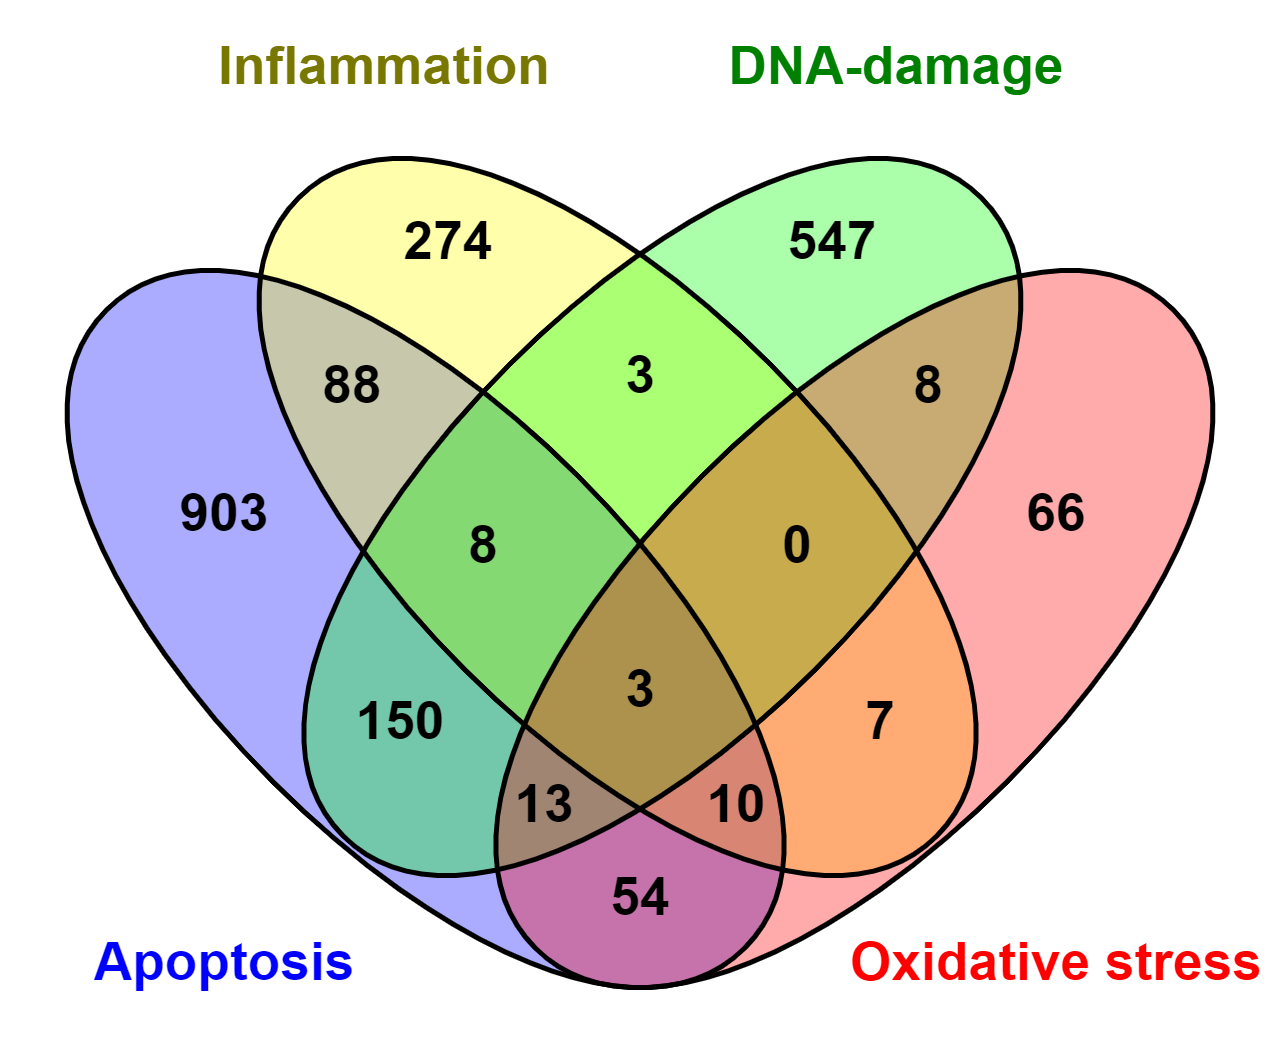
\includegraphics[height=6cm,keepaspectratio]{figA1.png}
\caption{Venn diagram showing the number of overlapping genes between the four GO-terms.
Venn diagram showing the number of overlapping genes between the four GO-terms; “apoptotic process”, “inflammation”, “cellular response to DNA damage stimulus”, “DNA damage and Oxidative stress”.
}
\label{fig:figA1}
\end{figure}

% Please add the following required packages to your document preamble:
% \usepackage{multirow}
\begin{table}[]
\caption{Table containing the number of pathways related to the four GO-terms. Based on either an overrepresentation analysis (p-value $<$ 0.05), 80\% gene overlap, 70\% gene overlap, 60\% gene overlap or 50\% gene overlap.
}
\label{tab:tabA2}
\resizebox{\columnwidth}{!}{%
\begin{tabular}{|l|c|c|c|c|c|}
\hline
\multirow{2}{*}{} & \multicolumn{5}{c|}{\textbf{Number of pathways   based on}} \\ \cline{2-6} 
 & \begin{tabular}[c]{@{}c@{}}ORA \\ (adjust p.value \textless 0.05)\end{tabular} & \begin{tabular}[c]{@{}c@{}}80\% \\ gene overlap\end{tabular} & \begin{tabular}[c]{@{}c@{}}70\% \\ gene overlap\end{tabular} & \begin{tabular}[c]{@{}c@{}}60\% \\ gene overlap\end{tabular} & \begin{tabular}[c]{@{}c@{}}50\% \\ gene overlap\end{tabular} \\ \hline
\begin{tabular}[c]{@{}l@{}}apoptotic process \\ (GO:0006915)\end{tabular} & 401 & 11 & 15 & 31 & 66 \\ \hline
\begin{tabular}[c]{@{}l@{}}inflammatory response \\ (GO:0006954)\end{tabular} & 250 & 0 & 0 & 6 & 15 \\ \hline
\begin{tabular}[c]{@{}l@{}}DNA damage \\ (GO:0006974)\end{tabular} & 203 & 15 & 20 & 23 & 28 \\ \hline
\begin{tabular}[c]{@{}l@{}}oxidative stress \\ (GO:0006979)\end{tabular} & 205 & 1 & 1 & 1 & 1 \\ \hline
\end{tabular}%
}
\end{table}

\begin{figure}[ht!]
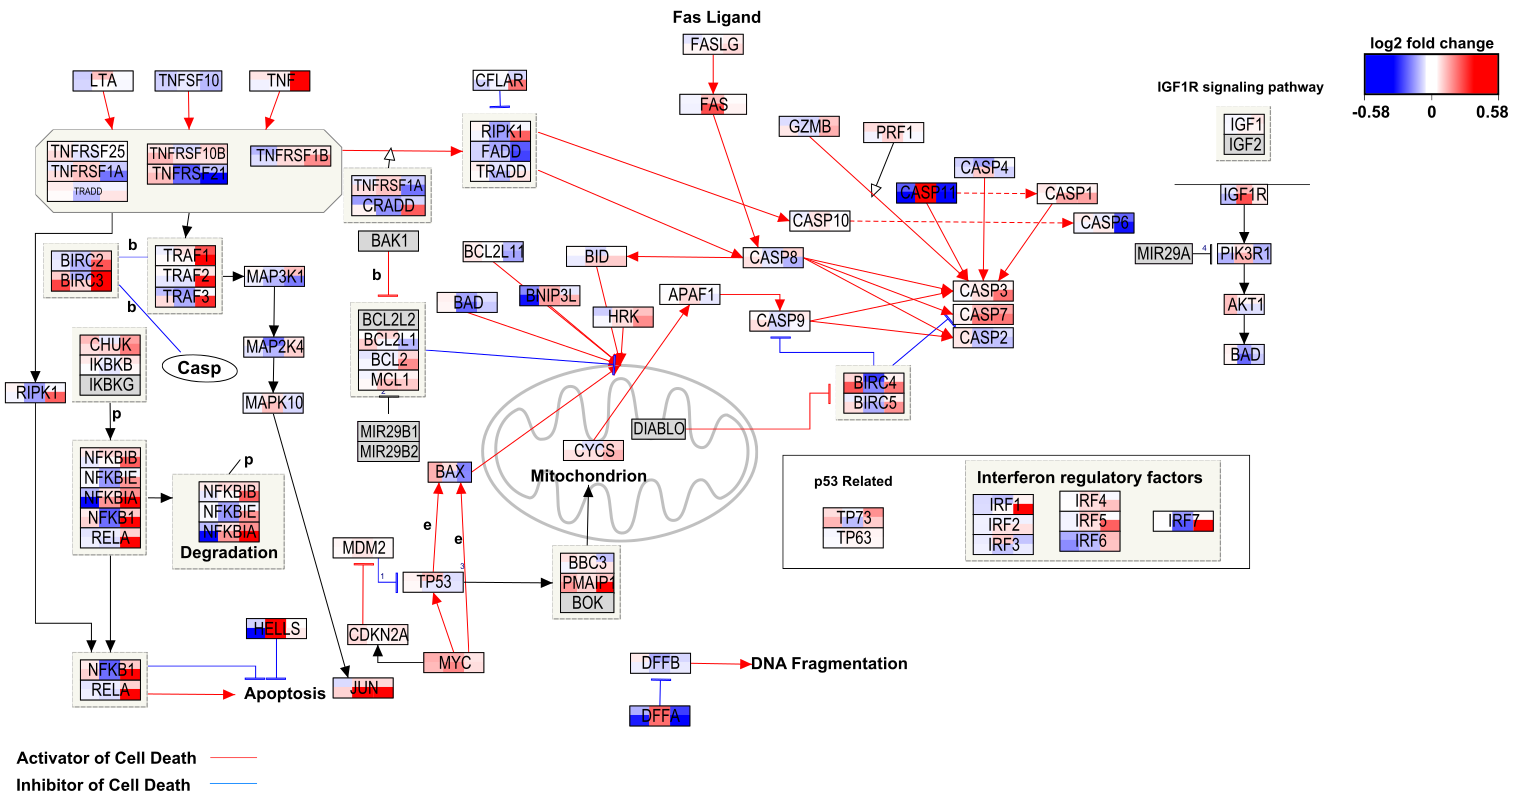
\includegraphics[height=7cm,keepaspectratio]{figA2.png}
\caption{Visualization of log fold change on the Apoptosis pathway (wikipathways:WP254) for all six conditions.
Cell lines are depicted from left to right as Caco2, SAE and THP1. The top row depicts the low concentration whereas the bottom row depicts the high concentration. Gradient goes from blue (log fold change $<$ -0.58) via white (log fold change = 0.0) to red (log fold change $>$ 0.58).
}
\label{fig:figA3}
\end{figure}

\begin{figure}[ht!]
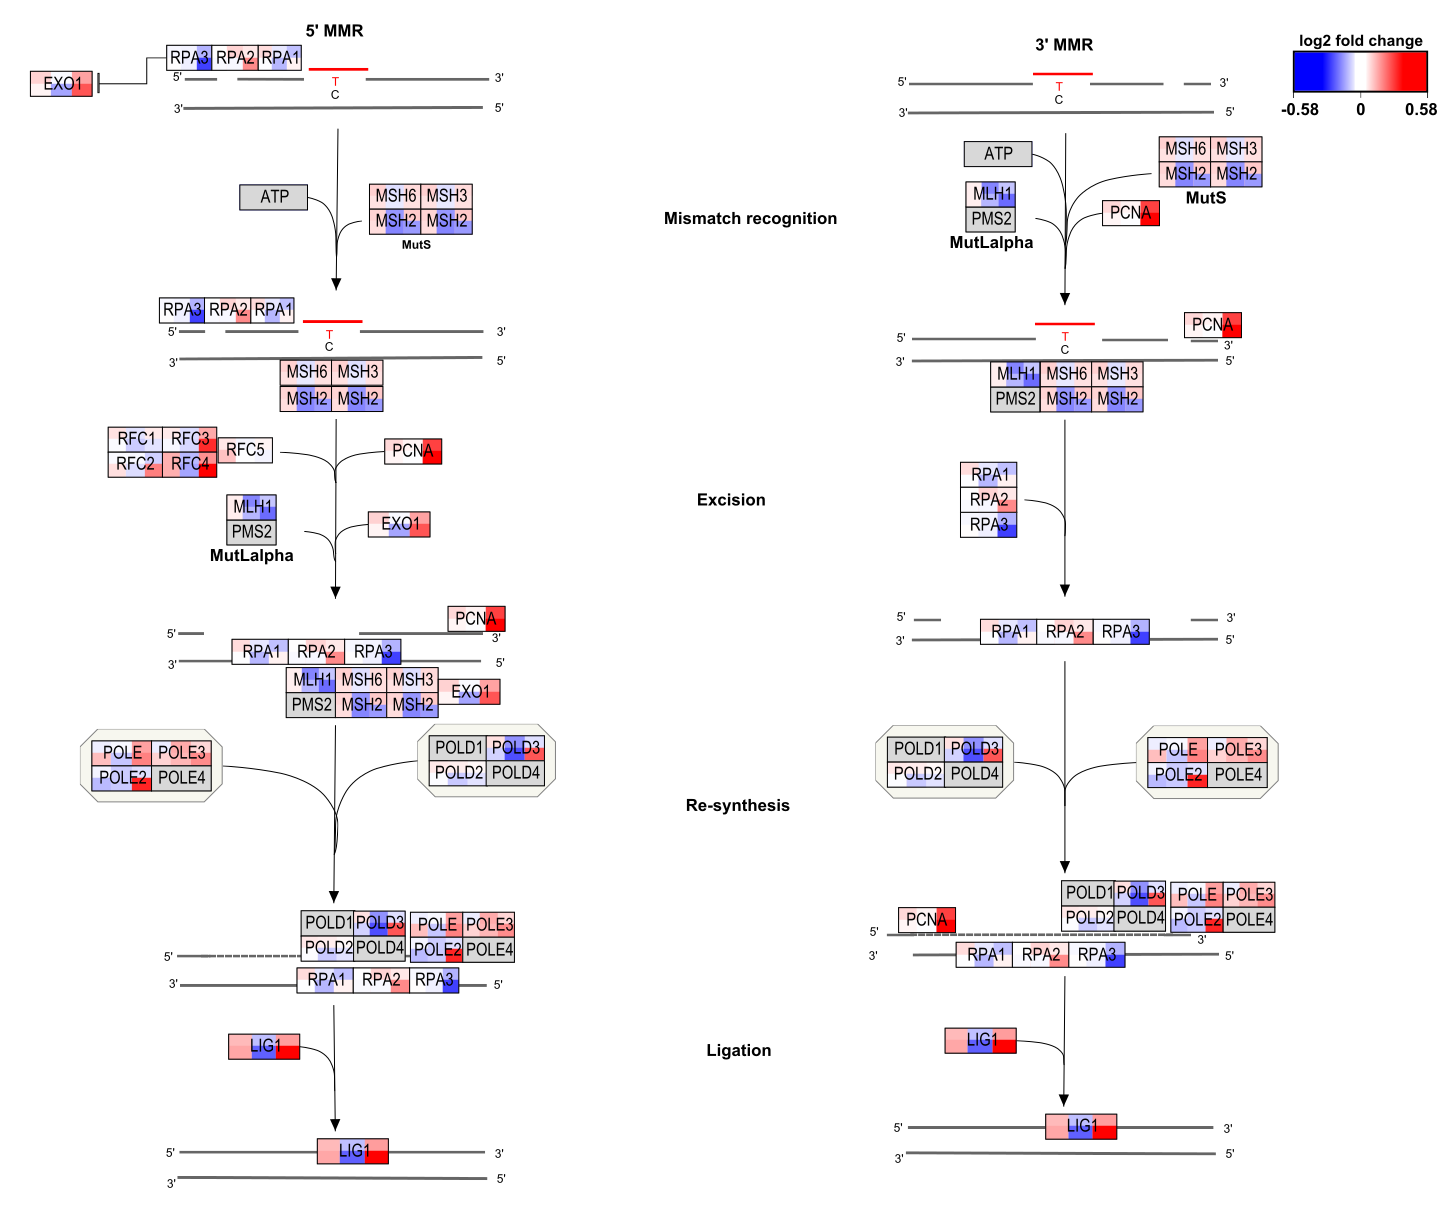
\includegraphics[height=10cm]{figA3.png}
\caption{Visualization of log fold change on the DNA Mismatch Repair pathway (wikipathways:WP531) for all six conditions.
Cell lines are depicted from left to right as Caco2, SAE and THP1. The top row depicts the low concentration whereas the bottom row depicts the high concentration. Gradient goes from blue (log fold change $<$ -0.58) via white (log fold change = 0.0) to red (log fold change $>$ 0.58).
}
\label{fig:figA4}
\end{figure}

% Please add the following required packages to your document preamble:
% \usepackage[table,xcdraw]{xcolor}
% If you use beamer only pass "xcolor=table" option, i.e. \documentclass[xcolor=table]{beamer}
\begin{table}[]
\caption{List of Gene Ontology (GO) evidence annotation codes which were used to remove genes related to the four GO-terms with these annotations (bottom part). Additionally, the annotation codes that were present are shown (top part).}
\label{tab:tabA5}
\resizebox{\columnwidth}{!}{%
\begin{tabular}{lll}
\multicolumn{1}{c}{{\color[HTML]{000000} \textbf{Abbreviation}}} & \multicolumn{1}{c}{{\color[HTML]{000000} \textbf{Full name}}} & \multicolumn{1}{c}{{\color[HTML]{000000} \textbf{Category}}} \\
\rowcolor[HTML]{C0C0C0} 
IBA                                                              & Inferred from Biological aspect of Ancestor                   & Phylogenetically-inferred annotations                        \\
IC                                                               & Inferred by Curator                                           & Curator statement evidence codes                             \\
\rowcolor[HTML]{C0C0C0} 
IDA                                                              & Inferred from Direct Assay                                    & Experimental evidence codes                                  \\
IEP                                                              & Inferred from Expression Pattern                              & Experimental evidence codes                                  \\
\rowcolor[HTML]{C0C0C0} 
IGI                                                              & Inferred from Genetic Interaction                             & Experimental evidence codes                                  \\
IMP                                                              & Inferred from Mutant Phenotype                                & Experimental evidence codes                                  \\
\rowcolor[HTML]{C0C0C0} 
IPI                                                              & Inferred from Physical Interaction                            & Experimental evidence codes                                  \\
TAS                                                              & Traceable Author Statement                                    & Author statement evidence codes                              \\
\multicolumn{3}{c}{\textbf{Removed annotations}}                                                                                                                                                \\
\rowcolor[HTML]{C0C0C0} 
ND                                                               & No Biological Data Available                                  & Curator statement evidence codes                             \\
NAS                                                              & Non-traceable Author Statement                                & Author statement evidence codes                              \\
\rowcolor[HTML]{C0C0C0} 
IEA                                                              & Inferred from Electronic Annotation                           & Electronic annotation evidence code                          \\
ISS                                                              & Inferred from Sequence or structural Similarity               & Computational analysis evidence codes                        \\
\rowcolor[HTML]{C0C0C0} 
ISO                                                              & Inferred from Sequence Orthology                              & Computational analysis evidence codes                        \\
ISA                                                              & Inferred from Sequence Alignment                              & Computational analysis evidence codes                        \\
\rowcolor[HTML]{C0C0C0} 
ISM                                                              & Inferred from Sequence Model                                  & Computational analysis evidence codes                        \\
IGC                                                              & Inferred from Genomic Context                                 & Computational analysis evidence codes                        \\
\rowcolor[HTML]{C0C0C0} 
RCA                                                              & Inferred from Reviewed Computational Analysis & Computational analysis evidence codes
\end{tabular}%
}
\end{table}


%The appendix is an optional section that can contain details and data supplemental to the main text---for example, explanations of experimental details that would disrupt the flow of the main text but nonetheless remain crucial to understanding and reproducing the research shown; figures of replicates for experiments of which representative data are shown in the main text can be added here if brief, or as Supplementary Data. Mathematical proofs of results not central to the paper can be added as an appendix.

%\section{}
%All appendix sections must be cited in the main text. In the appendices, Figures, Tables, etc. should be labeled, starting with ``A''---e.g., Figure A1, Figure A2, etc. 

%%%%%%%%%%%%%%%%%%%%%%%%%%%%%%%%%%%%%%%%%%
\end{paracol}
%%%%%%%%%%%%%%%%%%%%%%%%%%%%%%%%%%%%%%%%%%
\reftitle{References}

% Please provide either the correct journal abbreviation (e.g. according to the “List of Title Word Abbreviations” http://www.issn.org/services/online-services/access-to-the-ltwa/) or the full name of the journal.
% Citations and References in Supplementary files are permitted provided that they also appear in the reference list here. 

%=====================================
% References, variant A: external bibliography
%=====================================
\externalbibliography{yes}
\bibliography{references}

%%%%%%%%%%%%%%%%%%%%%%%%%%%%%%%%%%%%%%%%%%
%% for journal Sci
%\reviewreports{\\
%Reviewer 1 comments and authors’ response\\
%Reviewer 2 comments and authors’ response\\
%Reviewer 3 comments and authors’ response
%}
%%%%%%%%%%%%%%%%%%%%%%%%%%%%%%%%%%%%%%%%%%
\end{document}

